\documentclass{whiteboard}
\begin{document}
\begin{frame}[plain,t]
\bbcover{OBI 2008 - Nível 2: Fase 1}{Telefone}{Prof. Edson Alves}{Faculdade UnB Gama}

\end{frame}
\begin{frame}[plain,t]
\vspace*{\fill}

\bbtext{As primeiras redes públicas de telefonia foram construídas pela AT\&T; no começo do século XX. Elas permitiam que seus assinantes conversassem com a ajuda de uma telefonista, que conectava as linhas dos assinantes com um cabo especial.}

\vspace{0.1in}

\bbtext{Essas redes evoluíram muito desde então, com a ajuda de vários avanços tecnológicos. Hoje em dia, essas redes atendem centenas de milhões de assinantes; ao invés de falar diretamente com uma telefonista, você pode simplesmente discar o número da pessoa desejada no telefone.}

\vspace{0.1in}

\bbtext{Cada assinante recebe um número de telefone -- por exemplo, 55-98-234-5678. Qualquer pessoa que discar esse número consegue então falar com a pessoa do outro lado da linha. Os hifens no número de telefone são só para facilitar a leitura, e não são discados no telefone.}

\vspace{0.1in}

\bbtext{Para que fique mais fácil de se lembrar de um número de telefone, muitas companhias divulgam números que contém letras no lugar de dígitos. Para convertê-los de volta para dígitos, a maioria dos telefones tem letras nas suas teclas:}

\vspace*{\fill}
\end{frame}
\begin{frame}[plain,t]
\vspace*{\fill}

\begin{center}
\includegraphics[scale=0.8]{telefone.png}
\end{center}

\bbtext{Ao invés de discar uma letra, disca-se a tecla que contém aquela letra. Por exemplo, se você quiser discar o número 0800-FALE-SBC, você na realidade discaria 0800-3253-722.}

\vspace{0.1in}

\bbtext{A sua avó tem reclamado de problemas de vista -- em particular, ela não consegue mais enxergar as letrinhas nas teclas do telefone, e por isso queria que você fizesse um programa que convertesse as letras em um número de telefone para dígitos.}

\vspace*{\fill}
\end{frame}
\begin{frame}[plain,t]
\vspace*{\fill}

\bbbold{Entrada}

\vspace{0.2in}

\bbtext{A entrada contém um único conjunto de testes, que deve ser lido do \textit{dispositivo de entrada padrão} (normalmente
o teclado). A entrada é composta de apenas uma linha, contendo o número de telefone que deve ser traduzido.
O número de telefone contém entre 1 e 15 caracteres, que podem ser dígitos e `\texttt{0}' a `\texttt{9}', letras de `\texttt{A}' a `\texttt{Y}' e hífens
(`\texttt{-}').}

\vspace{0.2in}

\bbbold{Saída}

\vspace{0.2in}

\bbtext{Seu programa deve imprimir, na saída padrão, uma única linha, contendo o número de telefone com as letras
convertidas para dígitos. Hífens no número telefone devem ser mantidos no número de telefone de saída.}

\vspace*{\fill}
\end{frame}
\begin{frame}[plain,t]
\begin{tikzpicture}
\node[draw,opacity=0] at (0, 0) {x};
\node[draw,opacity=0] at (14, 8) {x};

	\node[anchor=west] (header) at (0, 7.0) { \bbbold{Exemplo de entrada e saída} };

\end{tikzpicture}
\end{frame}
\begin{frame}[plain,t]
\begin{tikzpicture}
\node[draw,opacity=0] at (0, 0) {x};
\node[draw,opacity=0] at (14, 8) {x};

	\node[anchor=west] (header) at (0, 7.0) { \bbbold{Exemplo de entrada e saída} };


	\node[anchor=west] (line1) at (1.0, 6.0) { \bbtext{\texttt{M1S-TU-R4} } };

\end{tikzpicture}
\end{frame}
\begin{frame}[plain,t]
\begin{tikzpicture}
\node[draw,opacity=0] at (0, 0) {x};
\node[draw,opacity=0] at (14, 8) {x};

	\node[anchor=west] (header) at (0, 7.0) { \bbbold{Exemplo de entrada e saída} };


	\node[anchor=west] (line1) at (1.0, 6.0) { \bbtext{\texttt{M1S-TU-R4} } };


	\draw[->,color=BBViolet] (2.15, 5.0) to  (2.15, 5.75);

	\node[] (r) at (2.75, 4.75) { \footnotesize \bbcomment{Telefone com letras, números e hífens} };

\end{tikzpicture}
\end{frame}
\begin{frame}[plain,t]
\begin{tikzpicture}
\node[draw,opacity=0] at (0, 0) {x};
\node[draw,opacity=0] at (14, 8) {x};

	\node[anchor=west] (header) at (0, 7.0) { \bbbold{Exemplo de entrada e saída} };


	\node[anchor=west] (line1) at (1.0, 6.0) { \bbtext{\texttt{M1S-TU-R4} } };





	\node[] (line2) at (7.0, 4.0) { \bbtext{\Huge \texttt{M1S-TU-R4}} };

\end{tikzpicture}
\end{frame}
\begin{frame}[plain,t]
\begin{tikzpicture}
\node[draw,opacity=0] at (0, 0) {x};
\node[draw,opacity=0] at (14, 8) {x};

	\node[anchor=west] (header) at (0, 7.0) { \bbbold{Exemplo de entrada e saída} };


	\node[anchor=west] (line1) at (1.0, 6.0) { \bbtext{\texttt{M1S-TU-R4} } };


	\draw[->,color=BBBlack,-latex,thick] (5.15, 3.6) to  (5.15, 2.85);

	\node[] (r) at (5.15, 2.5) { \bboutput{6} };


	\node[] (line2) at (7.0, 4.0) { \bbtext{\Huge \texttt{M1S-TU-R4}} };




\end{tikzpicture}
\end{frame}
\begin{frame}[plain,t]
\begin{tikzpicture}
\node[draw,opacity=0] at (0, 0) {x};
\node[draw,opacity=0] at (14, 8) {x};

	\node[anchor=west] (header) at (0, 7.0) { \bbbold{Exemplo de entrada e saída} };


	\node[anchor=west] (line1) at (1.0, 6.0) { \bbtext{\texttt{M1S-TU-R4} } };


	\draw[->,color=BBBlack,-latex,thick] (6.05, 3.6) to  (6.05, 2.85);

	\node[] (r) at (6.05, 2.5) { \bboutput{7} };


	\node[] (line2) at (7.0, 4.0) { \bbtext{\Huge \texttt{M1S-TU-R4}} };





\end{tikzpicture}
\end{frame}
\begin{frame}[plain,t]
\begin{tikzpicture}
\node[draw,opacity=0] at (0, 0) {x};
\node[draw,opacity=0] at (14, 8) {x};

	\node[anchor=west] (header) at (0, 7.0) { \bbbold{Exemplo de entrada e saída} };


	\node[anchor=west] (line1) at (1.0, 6.0) { \bbtext{\texttt{M1S-TU-R4} } };


	\draw[->,color=BBBlack,-latex,thick] (6.975, 3.6) to  (6.975, 2.85);

	\node[] (r) at (6.975, 2.5) { \bboutput{8} };


	\node[] (line2) at (7.0, 4.0) { \bbtext{\Huge \texttt{M1S-TU-R4}} };






\end{tikzpicture}
\end{frame}
\begin{frame}[plain,t]
\begin{tikzpicture}
\node[draw,opacity=0] at (0, 0) {x};
\node[draw,opacity=0] at (14, 8) {x};

	\node[anchor=west] (header) at (0, 7.0) { \bbbold{Exemplo de entrada e saída} };


	\node[anchor=west] (line1) at (1.0, 6.0) { \bbtext{\texttt{M1S-TU-R4} } };


	\draw[->,color=BBBlack,-latex,thick] (7.425, 3.6) to  (7.425, 2.85);

	\node[] (r) at (7.425, 2.5) { \bboutput{8} };


	\node[] (line2) at (7.0, 4.0) { \bbtext{\Huge \texttt{M1S-TU-R4}} };







\end{tikzpicture}
\end{frame}
\begin{frame}[plain,t]
\begin{tikzpicture}
\node[draw,opacity=0] at (0, 0) {x};
\node[draw,opacity=0] at (14, 8) {x};

	\node[anchor=west] (header) at (0, 7.0) { \bbbold{Exemplo de entrada e saída} };


	\node[anchor=west] (line1) at (1.0, 6.0) { \bbtext{\texttt{M1S-TU-R4} } };


	\draw[->,color=BBBlack,-latex,thick] (8.35, 3.6) to  (8.35, 2.85);

	\node[] (r) at (8.35, 2.5) { \bboutput{7} };


	\node[] (line2) at (7.0, 4.0) { \bbtext{\Huge \texttt{M1S-TU-R4}} };








\end{tikzpicture}
\end{frame}
\begin{frame}[plain,t]
\begin{tikzpicture}
\node[draw,opacity=0] at (0, 0) {x};
\node[draw,opacity=0] at (14, 8) {x};

	\node[anchor=west] (title) at (0.0, 7.5) { \Large \bbbold{Solução} };

\end{tikzpicture}
\end{frame}
\begin{frame}[plain,t]
\begin{tikzpicture}
\node[draw,opacity=0] at (0, 0) {x};
\node[draw,opacity=0] at (14, 8) {x};

	\node[anchor=west] (title) at (0.0, 7.5) { \Large \bbbold{Solução} };


	\node[anchor=west] (a) at (1.0, 6.5) { $\star$ \bbtext{Como o número de caracteres $N$ não é dado na entrada, o telefone deve ser} };

	\node[anchor=west] (a1) at (0.5, 6.0) { \bbtext{lido como uma string} };

\end{tikzpicture}
\end{frame}
\begin{frame}[plain,t]
\begin{tikzpicture}
\node[draw,opacity=0] at (0, 0) {x};
\node[draw,opacity=0] at (14, 8) {x};

	\node[anchor=west] (title) at (0.0, 7.5) { \Large \bbbold{Solução} };


	\node[anchor=west] (a) at (1.0, 6.5) { $\star$ \bbtext{Como o número de caracteres $N$ não é dado na entrada, o telefone deve ser} };

	\node[anchor=west] (a1) at (0.5, 6.0) { \bbtext{lido como uma string} };


	\node[anchor=west] (b) at (1.0, 5.0) { $\star$ \bbtext{A função \code{c}{strlen()} pode ser usada para computar o valor de $N$} };

\end{tikzpicture}
\end{frame}
\begin{frame}[plain,t]
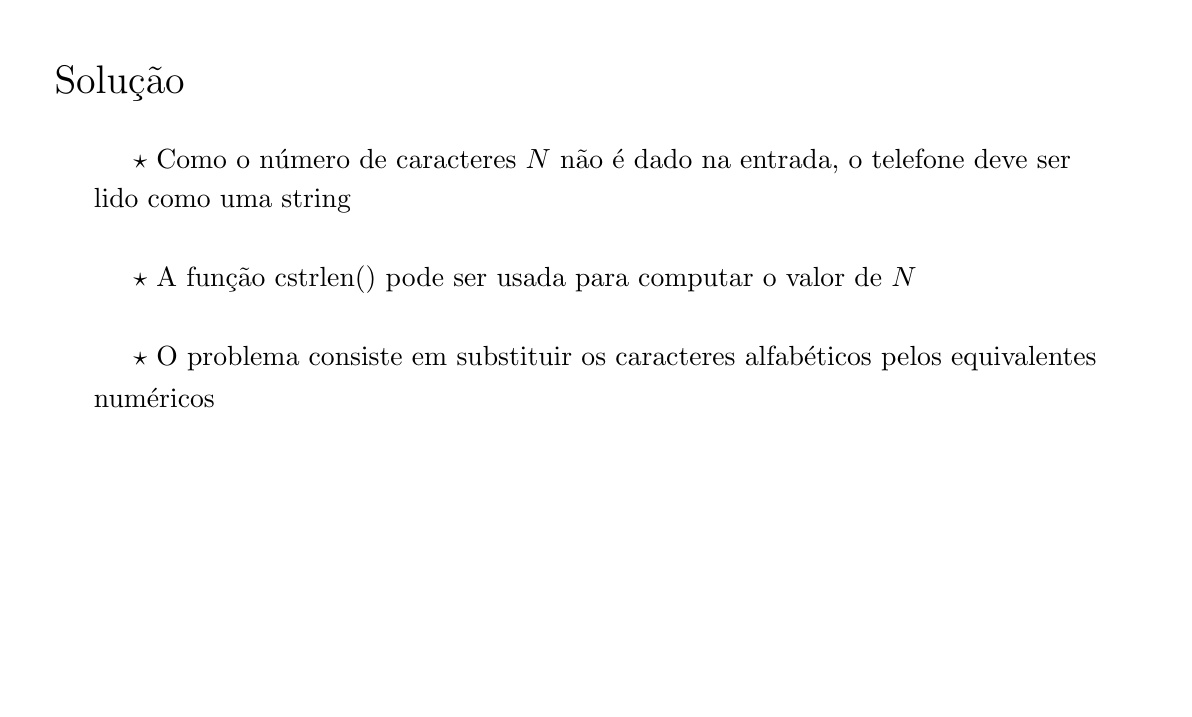
\begin{tikzpicture}
\node[draw,opacity=0] at (0, 0) {x};
\node[draw,opacity=0] at (14, 8) {x};

	\node[anchor=west] (title) at (0.0, 7.5) { \Large \bbbold{Solução} };


	\node[anchor=west] (a) at (1.0, 6.5) { $\star$ \bbtext{Como o número de caracteres $N$ não é dado na entrada, o telefone deve ser} };

	\node[anchor=west] (a1) at (0.5, 6.0) { \bbtext{lido como uma string} };


	\node[anchor=west] (b) at (1.0, 5.0) { $\star$ \bbtext{A função \code{c}{strlen()} pode ser usada para computar o valor de $N$} };


	\node[anchor=west] (c) at (1.0, 4.0) { $\star$ \bbtext{O problema consiste em substituir os caracteres alfabéticos pelos equivalentes} };

	\node[anchor=west] (c1) at (0.5, 3.5) { \bbtext{numéricos} };


\end{tikzpicture}
\end{frame}
\begin{frame}[plain,t]
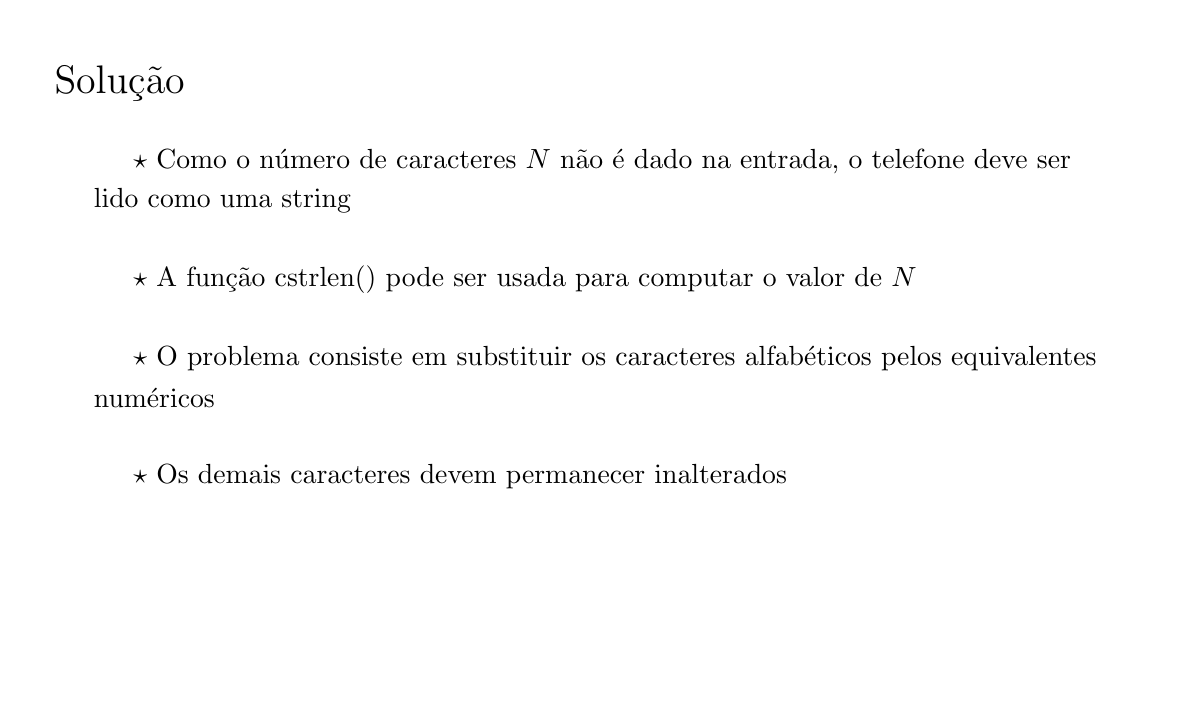
\begin{tikzpicture}
\node[draw,opacity=0] at (0, 0) {x};
\node[draw,opacity=0] at (14, 8) {x};

	\node[anchor=west] (title) at (0.0, 7.5) { \Large \bbbold{Solução} };


	\node[anchor=west] (a) at (1.0, 6.5) { $\star$ \bbtext{Como o número de caracteres $N$ não é dado na entrada, o telefone deve ser} };

	\node[anchor=west] (a1) at (0.5, 6.0) { \bbtext{lido como uma string} };


	\node[anchor=west] (b) at (1.0, 5.0) { $\star$ \bbtext{A função \code{c}{strlen()} pode ser usada para computar o valor de $N$} };


	\node[anchor=west] (c) at (1.0, 4.0) { $\star$ \bbtext{O problema consiste em substituir os caracteres alfabéticos pelos equivalentes} };

	\node[anchor=west] (c1) at (0.5, 3.5) { \bbtext{numéricos} };



	\node[anchor=west] (d) at (1.0, 2.5) { $\star$ \bbtext{Os demais caracteres devem permanecer inalterados} };

\end{tikzpicture}
\end{frame}
\begin{frame}[plain,t]
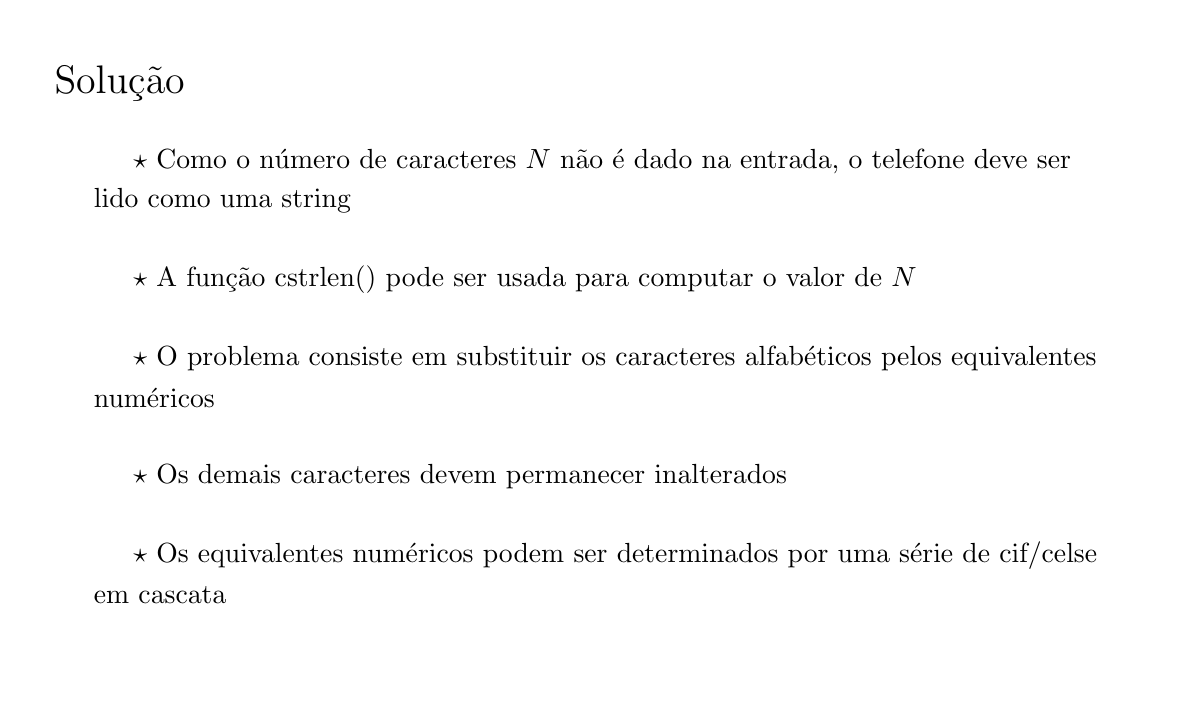
\begin{tikzpicture}
\node[draw,opacity=0] at (0, 0) {x};
\node[draw,opacity=0] at (14, 8) {x};

	\node[anchor=west] (title) at (0.0, 7.5) { \Large \bbbold{Solução} };


	\node[anchor=west] (a) at (1.0, 6.5) { $\star$ \bbtext{Como o número de caracteres $N$ não é dado na entrada, o telefone deve ser} };

	\node[anchor=west] (a1) at (0.5, 6.0) { \bbtext{lido como uma string} };


	\node[anchor=west] (b) at (1.0, 5.0) { $\star$ \bbtext{A função \code{c}{strlen()} pode ser usada para computar o valor de $N$} };


	\node[anchor=west] (c) at (1.0, 4.0) { $\star$ \bbtext{O problema consiste em substituir os caracteres alfabéticos pelos equivalentes} };

	\node[anchor=west] (c1) at (0.5, 3.5) { \bbtext{numéricos} };



	\node[anchor=west] (d) at (1.0, 2.5) { $\star$ \bbtext{Os demais caracteres devem permanecer inalterados} };


	\node[anchor=west] (e) at (1.0, 1.5) { $\star$ \bbtext{Os equivalentes numéricos podem ser determinados por uma série de \code{c}{if}/\code{c}{else}} };

	\node[anchor=west] (e1) at (0.5, 1.0) { \bbtext{em cascata} };

\end{tikzpicture}
\end{frame}
\begin{frame}[plain,t]
\begin{tikzpicture}
\node[draw,opacity=0] at (0, 0) {x};
\node[draw,opacity=0] at (14, 8) {x};

	\node[anchor=west] (line1) at (1.0, 8.0) { \inputsmallline{c}{1}{codes/solution.c} };



	\node[anchor=west] (line4) at (1.0, 6.86) { \inputsmallline{c}{4}{codes/solution.c} };

	\node[anchor=west] (line5) at (1.0, 6.48) { \inputsmallline{c}{5}{codes/solution.c} };


















	\draw[color=gray,dashed] (7.5, 8) -- (7.5, 0) -- cycle;










	\node[anchor=west] (line33) at (8.0, 3.81) { \inputsmallline{c}{33}{codes/solution.c} };

	\node[anchor=west] (line34) at (8.0, 3.43) { \inputsmallline{c}{34}{codes/solution.c} };


\end{tikzpicture}
\end{frame}
\begin{frame}[plain,t]
\begin{tikzpicture}
\node[draw,opacity=0] at (0, 0) {x};
\node[draw,opacity=0] at (14, 8) {x};

	\node[anchor=west] (line1) at (1.0, 8.0) { \inputsmallline{c}{1}{codes/solution.c} };



	\node[anchor=west] (line4) at (1.0, 6.86) { \inputsmallline{c}{4}{codes/solution.c} };

	\node[anchor=west] (line5) at (1.0, 6.48) { \inputsmallline{c}{5}{codes/solution.c} };

	\node[anchor=west] (line6) at (1.0, 6.1) { \inputsmallline{c}{6}{codes/solution.c} };

	\node[anchor=west] (line7) at (1.0, 5.71) { \inputsmallline{c}{7}{codes/solution.c} };
















	\draw[color=gray,dashed] (7.5, 8) -- (7.5, 0) -- cycle;










	\node[anchor=west] (line33) at (8.0, 3.81) { \inputsmallline{c}{33}{codes/solution.c} };

	\node[anchor=west] (line34) at (8.0, 3.43) { \inputsmallline{c}{34}{codes/solution.c} };




\end{tikzpicture}
\end{frame}
\begin{frame}[plain,t]
\begin{tikzpicture}
\node[draw,opacity=0] at (0, 0) {x};
\node[draw,opacity=0] at (14, 8) {x};

	\node[anchor=west] (line1) at (1.0, 8.0) { \inputsmallline{c}{1}{codes/solution.c} };

	\node[anchor=west] (line2) at (1.0, 7.62) { \inputsmallline{c}{2}{codes/solution.c} };


	\node[anchor=west] (line4) at (1.0, 6.86) { \inputsmallline{c}{4}{codes/solution.c} };

	\node[anchor=west] (line5) at (1.0, 6.48) { \inputsmallline{c}{5}{codes/solution.c} };

	\node[anchor=west] (line6) at (1.0, 6.1) { \inputsmallline{c}{6}{codes/solution.c} };

	\node[anchor=west] (line7) at (1.0, 5.71) { \inputsmallline{c}{7}{codes/solution.c} };


	\node[anchor=west] (line9) at (1.0, 4.95) { \inputsmallline{c}{9}{codes/solution.c} };














	\draw[color=gray,dashed] (7.5, 8) -- (7.5, 0) -- cycle;










	\node[anchor=west] (line33) at (8.0, 3.81) { \inputsmallline{c}{33}{codes/solution.c} };

	\node[anchor=west] (line34) at (8.0, 3.43) { \inputsmallline{c}{34}{codes/solution.c} };






\end{tikzpicture}
\end{frame}
\begin{frame}[plain,t]
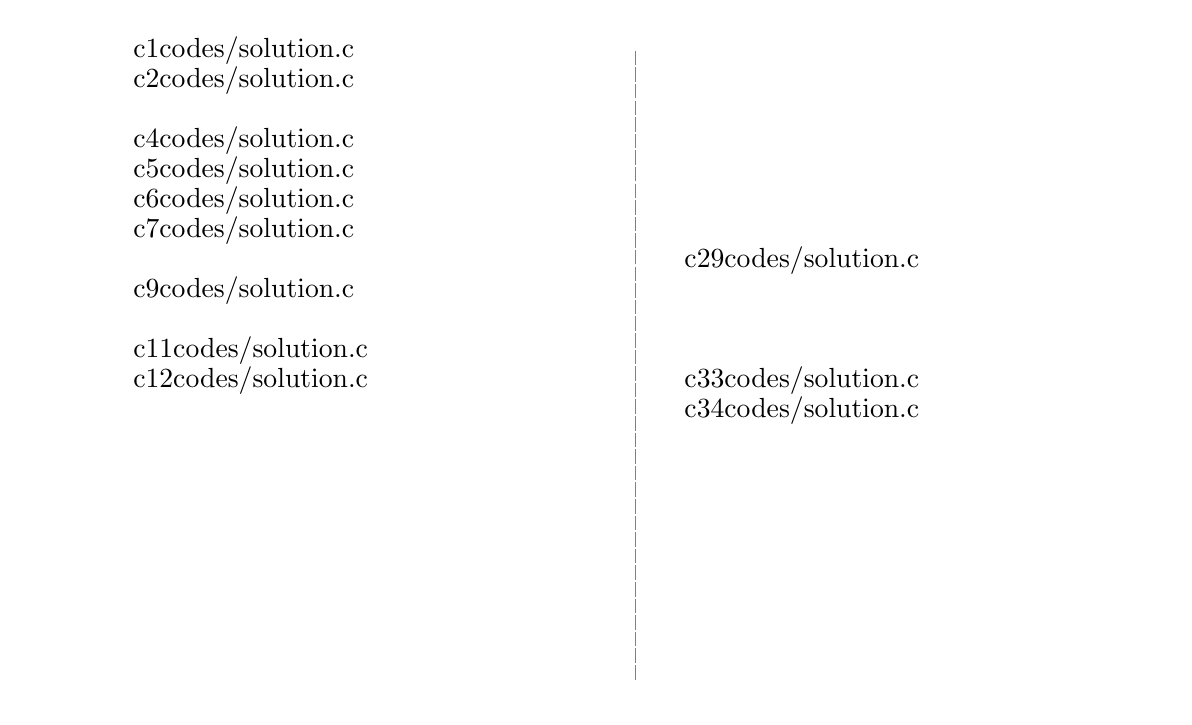
\begin{tikzpicture}
\node[draw,opacity=0] at (0, 0) {x};
\node[draw,opacity=0] at (14, 8) {x};

	\node[anchor=west] (line1) at (1.0, 8.0) { \inputsmallline{c}{1}{codes/solution.c} };

	\node[anchor=west] (line2) at (1.0, 7.62) { \inputsmallline{c}{2}{codes/solution.c} };


	\node[anchor=west] (line4) at (1.0, 6.86) { \inputsmallline{c}{4}{codes/solution.c} };

	\node[anchor=west] (line5) at (1.0, 6.48) { \inputsmallline{c}{5}{codes/solution.c} };

	\node[anchor=west] (line6) at (1.0, 6.1) { \inputsmallline{c}{6}{codes/solution.c} };

	\node[anchor=west] (line7) at (1.0, 5.71) { \inputsmallline{c}{7}{codes/solution.c} };


	\node[anchor=west] (line9) at (1.0, 4.95) { \inputsmallline{c}{9}{codes/solution.c} };


	\node[anchor=west] (line11) at (1.0, 4.19) { \inputsmallline{c}{11}{codes/solution.c} };

	\node[anchor=west] (line12) at (1.0, 3.81) { \inputsmallline{c}{12}{codes/solution.c} };











	\draw[color=gray,dashed] (7.5, 8) -- (7.5, 0) -- cycle;






	\node[anchor=west] (line29) at (8.0, 5.33) { \inputsmallline{c}{29}{codes/solution.c} };




	\node[anchor=west] (line33) at (8.0, 3.81) { \inputsmallline{c}{33}{codes/solution.c} };

	\node[anchor=west] (line34) at (8.0, 3.43) { \inputsmallline{c}{34}{codes/solution.c} };








\end{tikzpicture}
\end{frame}
\begin{frame}[plain,t]
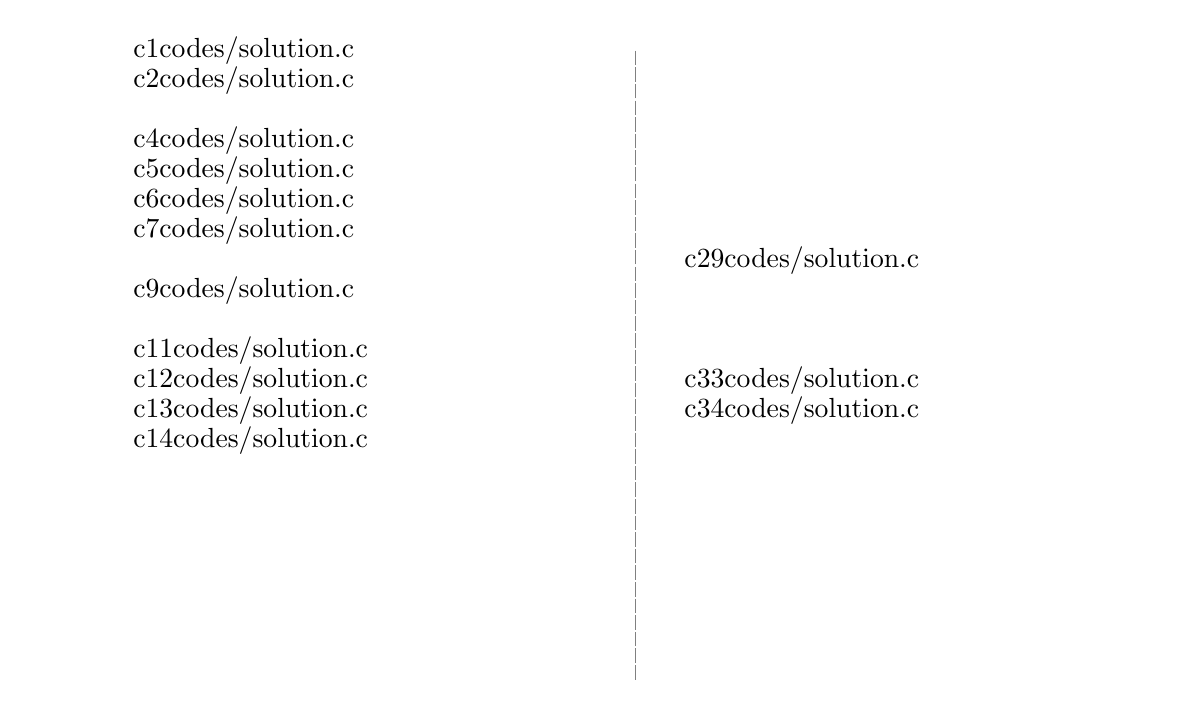
\begin{tikzpicture}
\node[draw,opacity=0] at (0, 0) {x};
\node[draw,opacity=0] at (14, 8) {x};

	\node[anchor=west] (line1) at (1.0, 8.0) { \inputsmallline{c}{1}{codes/solution.c} };

	\node[anchor=west] (line2) at (1.0, 7.62) { \inputsmallline{c}{2}{codes/solution.c} };


	\node[anchor=west] (line4) at (1.0, 6.86) { \inputsmallline{c}{4}{codes/solution.c} };

	\node[anchor=west] (line5) at (1.0, 6.48) { \inputsmallline{c}{5}{codes/solution.c} };

	\node[anchor=west] (line6) at (1.0, 6.1) { \inputsmallline{c}{6}{codes/solution.c} };

	\node[anchor=west] (line7) at (1.0, 5.71) { \inputsmallline{c}{7}{codes/solution.c} };


	\node[anchor=west] (line9) at (1.0, 4.95) { \inputsmallline{c}{9}{codes/solution.c} };


	\node[anchor=west] (line11) at (1.0, 4.19) { \inputsmallline{c}{11}{codes/solution.c} };

	\node[anchor=west] (line12) at (1.0, 3.81) { \inputsmallline{c}{12}{codes/solution.c} };

	\node[anchor=west] (line13) at (1.0, 3.43) { \inputsmallline{c}{13}{codes/solution.c} };

	\node[anchor=west] (line14) at (1.0, 3.05) { \inputsmallline{c}{14}{codes/solution.c} };









	\draw[color=gray,dashed] (7.5, 8) -- (7.5, 0) -- cycle;






	\node[anchor=west] (line29) at (8.0, 5.33) { \inputsmallline{c}{29}{codes/solution.c} };




	\node[anchor=west] (line33) at (8.0, 3.81) { \inputsmallline{c}{33}{codes/solution.c} };

	\node[anchor=west] (line34) at (8.0, 3.43) { \inputsmallline{c}{34}{codes/solution.c} };










\end{tikzpicture}
\end{frame}
\begin{frame}[plain,t]
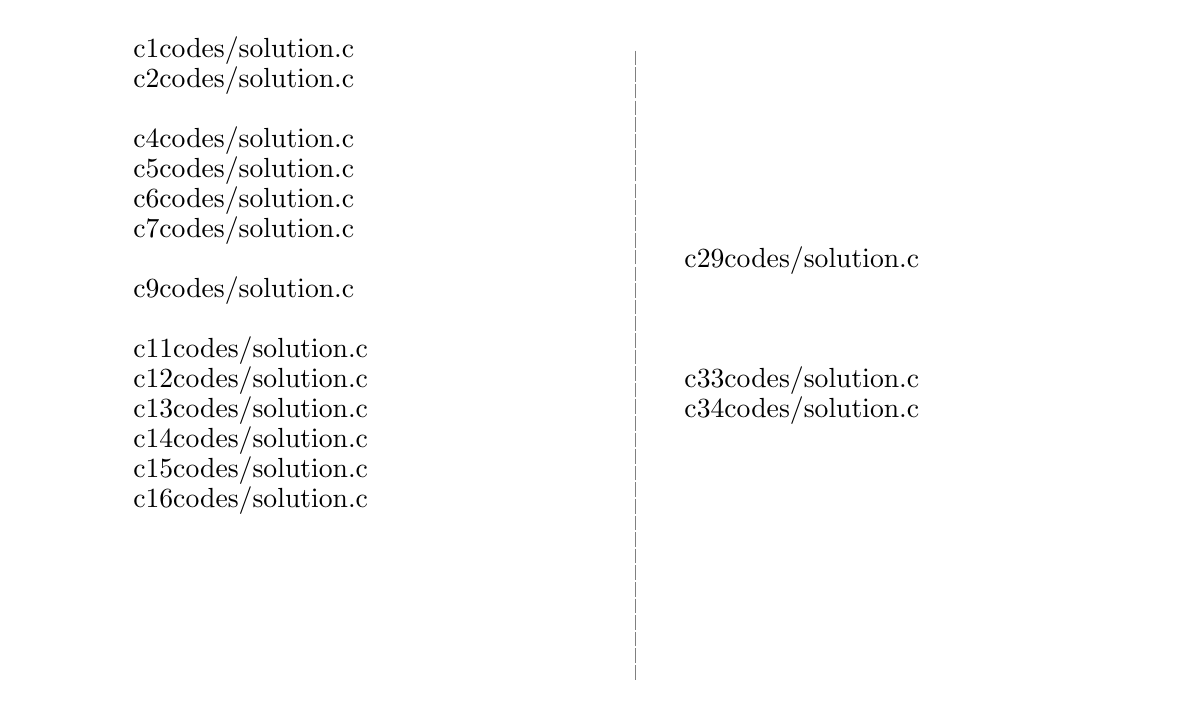
\begin{tikzpicture}
\node[draw,opacity=0] at (0, 0) {x};
\node[draw,opacity=0] at (14, 8) {x};

	\node[anchor=west] (line1) at (1.0, 8.0) { \inputsmallline{c}{1}{codes/solution.c} };

	\node[anchor=west] (line2) at (1.0, 7.62) { \inputsmallline{c}{2}{codes/solution.c} };


	\node[anchor=west] (line4) at (1.0, 6.86) { \inputsmallline{c}{4}{codes/solution.c} };

	\node[anchor=west] (line5) at (1.0, 6.48) { \inputsmallline{c}{5}{codes/solution.c} };

	\node[anchor=west] (line6) at (1.0, 6.1) { \inputsmallline{c}{6}{codes/solution.c} };

	\node[anchor=west] (line7) at (1.0, 5.71) { \inputsmallline{c}{7}{codes/solution.c} };


	\node[anchor=west] (line9) at (1.0, 4.95) { \inputsmallline{c}{9}{codes/solution.c} };


	\node[anchor=west] (line11) at (1.0, 4.19) { \inputsmallline{c}{11}{codes/solution.c} };

	\node[anchor=west] (line12) at (1.0, 3.81) { \inputsmallline{c}{12}{codes/solution.c} };

	\node[anchor=west] (line13) at (1.0, 3.43) { \inputsmallline{c}{13}{codes/solution.c} };

	\node[anchor=west] (line14) at (1.0, 3.05) { \inputsmallline{c}{14}{codes/solution.c} };

	\node[anchor=west] (line15) at (1.0, 2.67) { \inputsmallline{c}{15}{codes/solution.c} };

	\node[anchor=west] (line16) at (1.0, 2.29) { \inputsmallline{c}{16}{codes/solution.c} };







	\draw[color=gray,dashed] (7.5, 8) -- (7.5, 0) -- cycle;






	\node[anchor=west] (line29) at (8.0, 5.33) { \inputsmallline{c}{29}{codes/solution.c} };




	\node[anchor=west] (line33) at (8.0, 3.81) { \inputsmallline{c}{33}{codes/solution.c} };

	\node[anchor=west] (line34) at (8.0, 3.43) { \inputsmallline{c}{34}{codes/solution.c} };












\end{tikzpicture}
\end{frame}
\begin{frame}[plain,t]
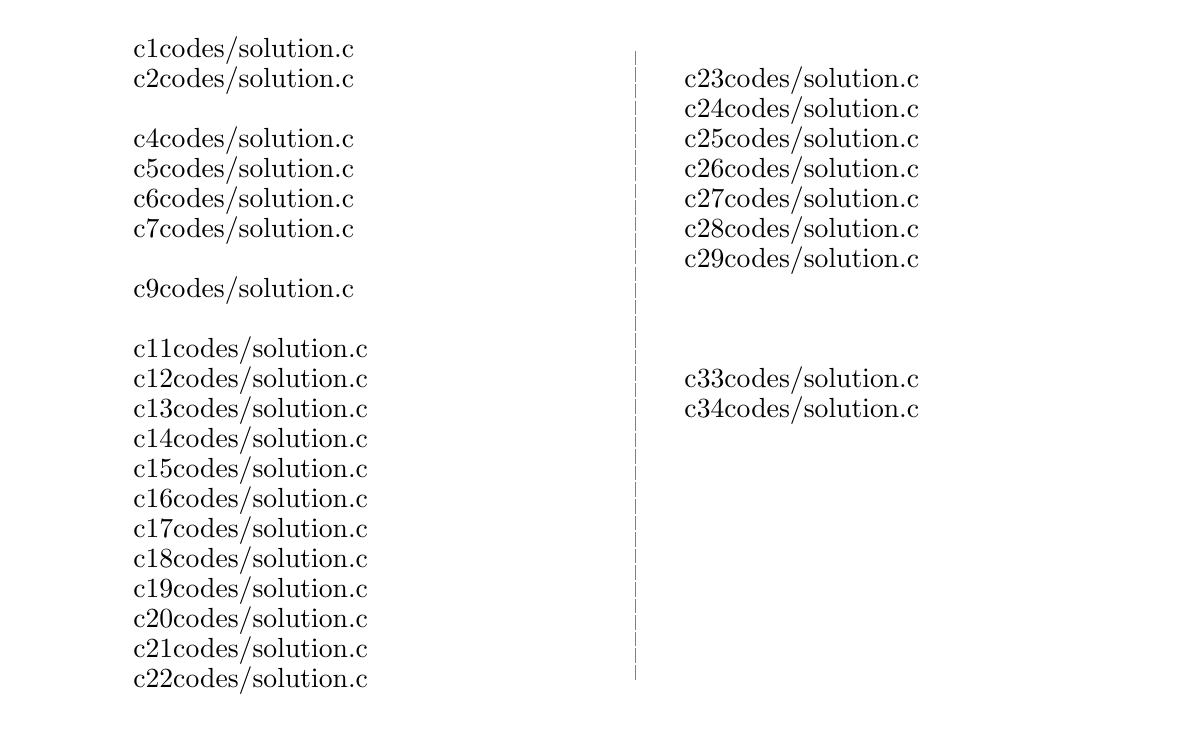
\begin{tikzpicture}
\node[draw,opacity=0] at (0, 0) {x};
\node[draw,opacity=0] at (14, 8) {x};

	\node[anchor=west] (line1) at (1.0, 8.0) { \inputsmallline{c}{1}{codes/solution.c} };

	\node[anchor=west] (line2) at (1.0, 7.62) { \inputsmallline{c}{2}{codes/solution.c} };


	\node[anchor=west] (line4) at (1.0, 6.86) { \inputsmallline{c}{4}{codes/solution.c} };

	\node[anchor=west] (line5) at (1.0, 6.48) { \inputsmallline{c}{5}{codes/solution.c} };

	\node[anchor=west] (line6) at (1.0, 6.1) { \inputsmallline{c}{6}{codes/solution.c} };

	\node[anchor=west] (line7) at (1.0, 5.71) { \inputsmallline{c}{7}{codes/solution.c} };


	\node[anchor=west] (line9) at (1.0, 4.95) { \inputsmallline{c}{9}{codes/solution.c} };


	\node[anchor=west] (line11) at (1.0, 4.19) { \inputsmallline{c}{11}{codes/solution.c} };

	\node[anchor=west] (line12) at (1.0, 3.81) { \inputsmallline{c}{12}{codes/solution.c} };

	\node[anchor=west] (line13) at (1.0, 3.43) { \inputsmallline{c}{13}{codes/solution.c} };

	\node[anchor=west] (line14) at (1.0, 3.05) { \inputsmallline{c}{14}{codes/solution.c} };

	\node[anchor=west] (line15) at (1.0, 2.67) { \inputsmallline{c}{15}{codes/solution.c} };

	\node[anchor=west] (line16) at (1.0, 2.29) { \inputsmallline{c}{16}{codes/solution.c} };

	\node[anchor=west] (line17) at (1.0, 1.9) { \inputsmallline{c}{17}{codes/solution.c} };

	\node[anchor=west] (line18) at (1.0, 1.52) { \inputsmallline{c}{18}{codes/solution.c} };

	\node[anchor=west] (line19) at (1.0, 1.14) { \inputsmallline{c}{19}{codes/solution.c} };

	\node[anchor=west] (line20) at (1.0, 0.76) { \inputsmallline{c}{20}{codes/solution.c} };

	\node[anchor=west] (line21) at (1.0, 0.38) { \inputsmallline{c}{21}{codes/solution.c} };

	\node[anchor=west] (line22) at (1.0, -0.0) { \inputsmallline{c}{22}{codes/solution.c} };

	\draw[color=gray,dashed] (7.5, 8) -- (7.5, 0) -- cycle;
	\node[anchor=west] (line23) at (8.0, 7.62) { \inputsmallline{c}{23}{codes/solution.c} };

	\node[anchor=west] (line24) at (8.0, 7.24) { \inputsmallline{c}{24}{codes/solution.c} };

	\node[anchor=west] (line25) at (8.0, 6.86) { \inputsmallline{c}{25}{codes/solution.c} };

	\node[anchor=west] (line26) at (8.0, 6.48) { \inputsmallline{c}{26}{codes/solution.c} };

	\node[anchor=west] (line27) at (8.0, 6.1) { \inputsmallline{c}{27}{codes/solution.c} };

	\node[anchor=west] (line28) at (8.0, 5.71) { \inputsmallline{c}{28}{codes/solution.c} };

	\node[anchor=west] (line29) at (8.0, 5.33) { \inputsmallline{c}{29}{codes/solution.c} };




	\node[anchor=west] (line33) at (8.0, 3.81) { \inputsmallline{c}{33}{codes/solution.c} };

	\node[anchor=west] (line34) at (8.0, 3.43) { \inputsmallline{c}{34}{codes/solution.c} };














\end{tikzpicture}
\end{frame}
\begin{frame}[plain,t]
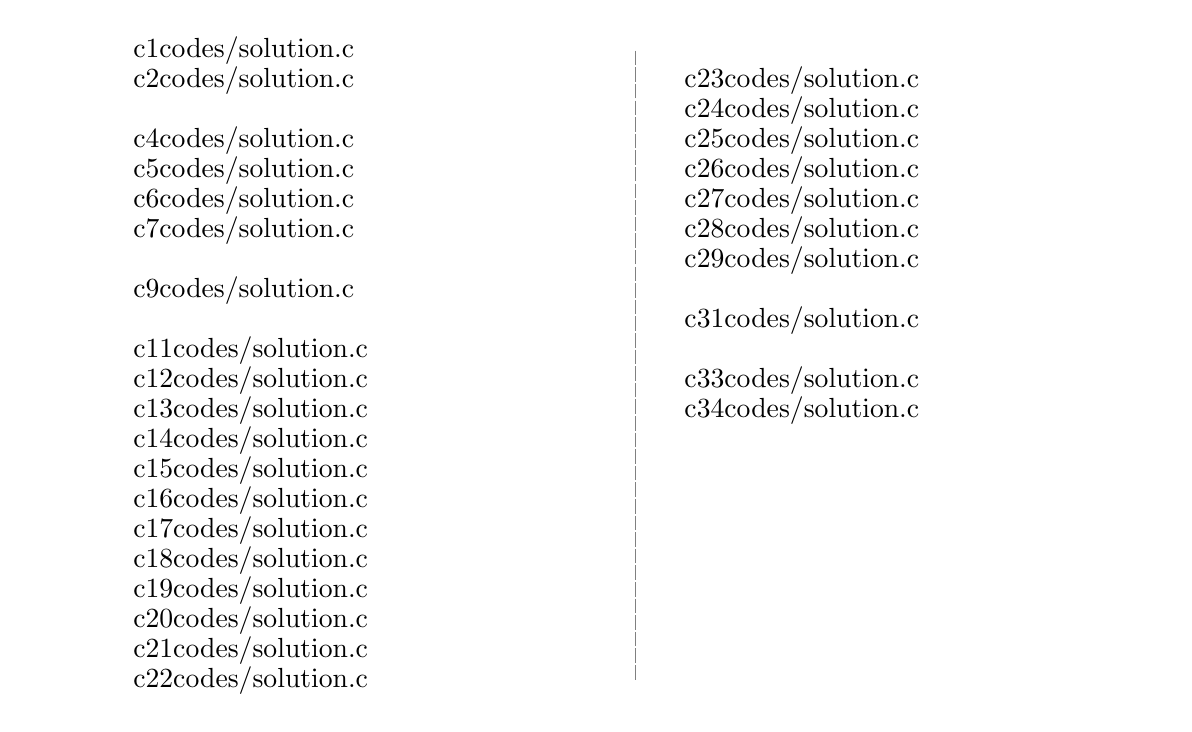
\begin{tikzpicture}
\node[draw,opacity=0] at (0, 0) {x};
\node[draw,opacity=0] at (14, 8) {x};

	\node[anchor=west] (line1) at (1.0, 8.0) { \inputsmallline{c}{1}{codes/solution.c} };

	\node[anchor=west] (line2) at (1.0, 7.62) { \inputsmallline{c}{2}{codes/solution.c} };


	\node[anchor=west] (line4) at (1.0, 6.86) { \inputsmallline{c}{4}{codes/solution.c} };

	\node[anchor=west] (line5) at (1.0, 6.48) { \inputsmallline{c}{5}{codes/solution.c} };

	\node[anchor=west] (line6) at (1.0, 6.1) { \inputsmallline{c}{6}{codes/solution.c} };

	\node[anchor=west] (line7) at (1.0, 5.71) { \inputsmallline{c}{7}{codes/solution.c} };


	\node[anchor=west] (line9) at (1.0, 4.95) { \inputsmallline{c}{9}{codes/solution.c} };


	\node[anchor=west] (line11) at (1.0, 4.19) { \inputsmallline{c}{11}{codes/solution.c} };

	\node[anchor=west] (line12) at (1.0, 3.81) { \inputsmallline{c}{12}{codes/solution.c} };

	\node[anchor=west] (line13) at (1.0, 3.43) { \inputsmallline{c}{13}{codes/solution.c} };

	\node[anchor=west] (line14) at (1.0, 3.05) { \inputsmallline{c}{14}{codes/solution.c} };

	\node[anchor=west] (line15) at (1.0, 2.67) { \inputsmallline{c}{15}{codes/solution.c} };

	\node[anchor=west] (line16) at (1.0, 2.29) { \inputsmallline{c}{16}{codes/solution.c} };

	\node[anchor=west] (line17) at (1.0, 1.9) { \inputsmallline{c}{17}{codes/solution.c} };

	\node[anchor=west] (line18) at (1.0, 1.52) { \inputsmallline{c}{18}{codes/solution.c} };

	\node[anchor=west] (line19) at (1.0, 1.14) { \inputsmallline{c}{19}{codes/solution.c} };

	\node[anchor=west] (line20) at (1.0, 0.76) { \inputsmallline{c}{20}{codes/solution.c} };

	\node[anchor=west] (line21) at (1.0, 0.38) { \inputsmallline{c}{21}{codes/solution.c} };

	\node[anchor=west] (line22) at (1.0, -0.0) { \inputsmallline{c}{22}{codes/solution.c} };

	\draw[color=gray,dashed] (7.5, 8) -- (7.5, 0) -- cycle;
	\node[anchor=west] (line23) at (8.0, 7.62) { \inputsmallline{c}{23}{codes/solution.c} };

	\node[anchor=west] (line24) at (8.0, 7.24) { \inputsmallline{c}{24}{codes/solution.c} };

	\node[anchor=west] (line25) at (8.0, 6.86) { \inputsmallline{c}{25}{codes/solution.c} };

	\node[anchor=west] (line26) at (8.0, 6.48) { \inputsmallline{c}{26}{codes/solution.c} };

	\node[anchor=west] (line27) at (8.0, 6.1) { \inputsmallline{c}{27}{codes/solution.c} };

	\node[anchor=west] (line28) at (8.0, 5.71) { \inputsmallline{c}{28}{codes/solution.c} };

	\node[anchor=west] (line29) at (8.0, 5.33) { \inputsmallline{c}{29}{codes/solution.c} };


	\node[anchor=west] (line31) at (8.0, 4.57) { \inputsmallline{c}{31}{codes/solution.c} };


	\node[anchor=west] (line33) at (8.0, 3.81) { \inputsmallline{c}{33}{codes/solution.c} };

	\node[anchor=west] (line34) at (8.0, 3.43) { \inputsmallline{c}{34}{codes/solution.c} };

















\end{tikzpicture}
\end{frame}
\begin{frame}[plain,t]
\begin{tikzpicture}
\node[draw,opacity=0] at (0, 0) {x};
\node[draw,opacity=0] at (14, 8) {x};

	\node[anchor=west] (title) at (0.0, 7.0) { \Large \bbbold{Bônus} };

\end{tikzpicture}
\end{frame}
\begin{frame}[plain,t]
\begin{tikzpicture}
\node[draw,opacity=0] at (0, 0) {x};
\node[draw,opacity=0] at (14, 8) {x};

	\node[anchor=west] (title) at (0.0, 7.0) { \Large \bbbold{Bônus} };


	\node[anchor=west] (a) at (1.0, 6.0) { $\star$ \bbtext{Há uma solução alternativa para este problema} };

\end{tikzpicture}
\end{frame}
\begin{frame}[plain,t]
\begin{tikzpicture}
\node[draw,opacity=0] at (0, 0) {x};
\node[draw,opacity=0] at (14, 8) {x};

	\node[anchor=west] (title) at (0.0, 7.0) { \Large \bbbold{Bônus} };


	\node[anchor=west] (a) at (1.0, 6.0) { $\star$ \bbtext{Há uma solução alternativa para este problema} };


	\node[anchor=west] (b) at (1.0, 5.0) { $\star$ \bbtext{Ela é baseada no código que um caractere ocupa na tabela ASCII e um vetor} };

	\node[anchor=west] (b1) at (0.5, 4.5) { \bbtext{auxiliar} };

\end{tikzpicture}
\end{frame}
\begin{frame}[plain,t]
\begin{tikzpicture}
\node[draw,opacity=0] at (0, 0) {x};
\node[draw,opacity=0] at (14, 8) {x};

	\node[anchor=west] (title) at (0.0, 7.0) { \Large \bbbold{Bônus} };


	\node[anchor=west] (a) at (1.0, 6.0) { $\star$ \bbtext{Há uma solução alternativa para este problema} };


	\node[anchor=west] (b) at (1.0, 5.0) { $\star$ \bbtext{Ela é baseada no código que um caractere ocupa na tabela ASCII e um vetor} };

	\node[anchor=west] (b1) at (0.5, 4.5) { \bbtext{auxiliar} };


	\node[anchor=west] (c) at (1.0, 3.5) { $\star$ \bbtext{As letras estão em ordem crescente na tabela ASCII} };

\end{tikzpicture}
\end{frame}
\begin{frame}[plain,t]
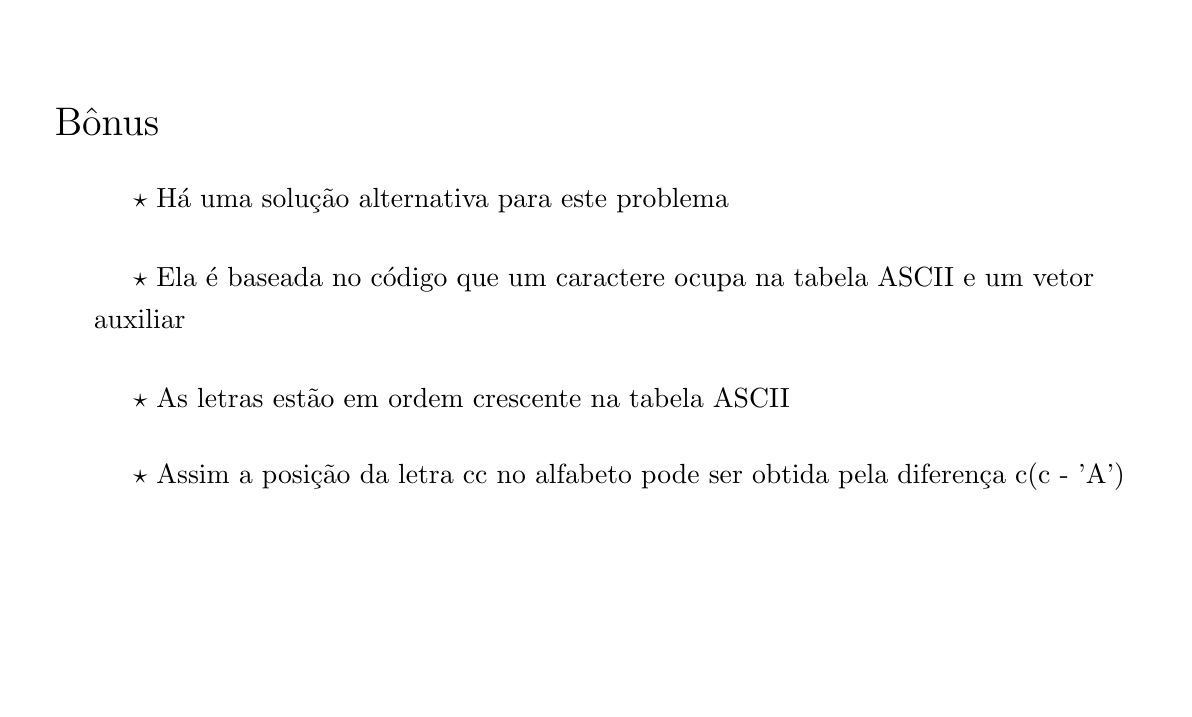
\begin{tikzpicture}
\node[draw,opacity=0] at (0, 0) {x};
\node[draw,opacity=0] at (14, 8) {x};

	\node[anchor=west] (title) at (0.0, 7.0) { \Large \bbbold{Bônus} };


	\node[anchor=west] (a) at (1.0, 6.0) { $\star$ \bbtext{Há uma solução alternativa para este problema} };


	\node[anchor=west] (b) at (1.0, 5.0) { $\star$ \bbtext{Ela é baseada no código que um caractere ocupa na tabela ASCII e um vetor} };

	\node[anchor=west] (b1) at (0.5, 4.5) { \bbtext{auxiliar} };


	\node[anchor=west] (c) at (1.0, 3.5) { $\star$ \bbtext{As letras estão em ordem crescente na tabela ASCII} };


	\node[anchor=west] (d) at (1.0, 2.5) { $\star$ \bbtext{Assim a posição da letra \code{c}{c} no alfabeto pode ser obtida pela diferença \code{c}{(c - 'A')}} };

\end{tikzpicture}
\end{frame}
\begin{frame}[plain,t]
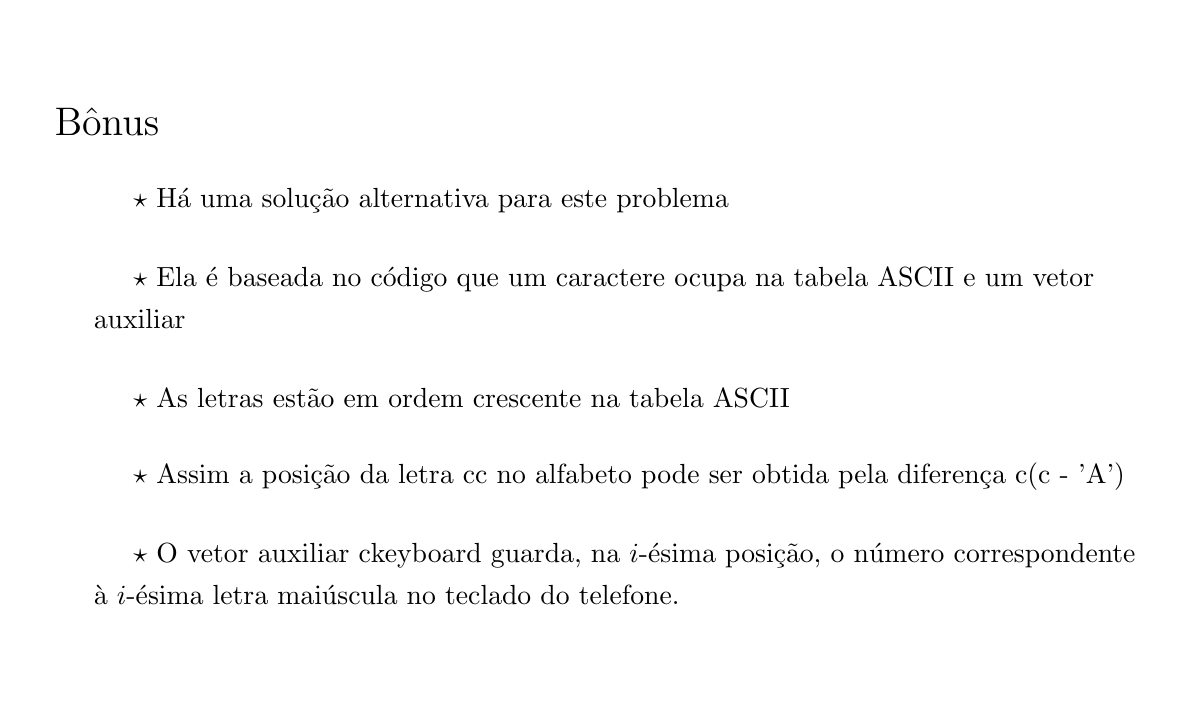
\begin{tikzpicture}
\node[draw,opacity=0] at (0, 0) {x};
\node[draw,opacity=0] at (14, 8) {x};

	\node[anchor=west] (title) at (0.0, 7.0) { \Large \bbbold{Bônus} };


	\node[anchor=west] (a) at (1.0, 6.0) { $\star$ \bbtext{Há uma solução alternativa para este problema} };


	\node[anchor=west] (b) at (1.0, 5.0) { $\star$ \bbtext{Ela é baseada no código que um caractere ocupa na tabela ASCII e um vetor} };

	\node[anchor=west] (b1) at (0.5, 4.5) { \bbtext{auxiliar} };


	\node[anchor=west] (c) at (1.0, 3.5) { $\star$ \bbtext{As letras estão em ordem crescente na tabela ASCII} };


	\node[anchor=west] (d) at (1.0, 2.5) { $\star$ \bbtext{Assim a posição da letra \code{c}{c} no alfabeto pode ser obtida pela diferença \code{c}{(c - 'A')}} };


	\node[anchor=west] (e) at (1.0, 1.5) { $\star$ \bbtext{O vetor auxiliar \code{c}{keyboard} guarda, na $i$-ésima posição, o número correspondente} };

	\node[anchor=west] (e1) at (0.5, 1.0) { \bbtext{à $i$-ésima letra maiúscula no teclado do telefone.} };

\end{tikzpicture}
\end{frame}
\begin{frame}[plain,t]
\begin{tikzpicture}
\node[draw,opacity=0] at (0, 0) {x};
\node[draw,opacity=0] at (14, 8) {x};

	\node[anchor=west] (line1) at (1.0, 8.0) { \inputline{c}{1}{codes/solution2.c} };


	\node[anchor=west] (line3) at (1.0, 7.2) { \inputline{c}{3}{codes/solution2.c} };


	\node[anchor=west] (line5) at (1.0, 6.4) { \inputline{c}{5}{codes/solution2.c} };

	\node[anchor=west] (line6) at (1.0, 6.0) { \inputline{c}{6}{codes/solution2.c} };

	\node[anchor=west] (line7) at (1.0, 5.6) { \inputline{c}{7}{codes/solution2.c} };

	\node[anchor=west] (line8) at (1.0, 5.2) { \inputline{c}{8}{codes/solution2.c} };


	\node[anchor=west] (line10) at (1.0, 4.4) { \inputline{c}{10}{codes/solution2.c} };










	\node[anchor=west] (line20) at (1.0, 0.4) { \inputline{c}{20}{codes/solution2.c} };

	\node[anchor=west] (line21) at (1.0, -0.0) { \inputline{c}{21}{codes/solution2.c} };


\end{tikzpicture}
\end{frame}
\begin{frame}[plain,t]
\begin{tikzpicture}
\node[draw,opacity=0] at (0, 0) {x};
\node[draw,opacity=0] at (14, 8) {x};

	\node[anchor=west] (line1) at (1.0, 8.0) { \inputline{c}{1}{codes/solution2.c} };


	\node[anchor=west] (line3) at (1.0, 7.2) { \inputline{c}{3}{codes/solution2.c} };


	\node[anchor=west] (line5) at (1.0, 6.4) { \inputline{c}{5}{codes/solution2.c} };

	\node[anchor=west] (line6) at (1.0, 6.0) { \inputline{c}{6}{codes/solution2.c} };

	\node[anchor=west] (line7) at (1.0, 5.6) { \inputline{c}{7}{codes/solution2.c} };

	\node[anchor=west] (line8) at (1.0, 5.2) { \inputline{c}{8}{codes/solution2.c} };


	\node[anchor=west] (line10) at (1.0, 4.4) { \inputline{c}{10}{codes/solution2.c} };


	\node[anchor=west] (line12) at (1.0, 3.6) { \inputline{c}{12}{codes/solution2.c} };








	\node[anchor=west] (line20) at (1.0, 0.4) { \inputline{c}{20}{codes/solution2.c} };

	\node[anchor=west] (line21) at (1.0, -0.0) { \inputline{c}{21}{codes/solution2.c} };




\end{tikzpicture}
\end{frame}
\begin{frame}[plain,t]

\begin{tikzpicture}
\node[draw,opacity=0] at (0, 0) {x};
\node[draw,opacity=0] at (14, 8) {x};

	\node[anchor=west] (line1) at (1.0, 8.0) { \inputline{c}{1}{codes/solution2.c} };


	\node[anchor=west] (line3) at (1.0, 7.2) { \inputline{c}{3}{codes/solution2.c} };


	\node[anchor=west] (line5) at (1.0, 6.4) { \inputline{c}{5}{codes/solution2.c} };

	\node[anchor=west] (line6) at (1.0, 6.0) { \inputline{c}{6}{codes/solution2.c} };

	\node[anchor=west] (line7) at (1.0, 5.6) { \inputline{c}{7}{codes/solution2.c} };

	\node[anchor=west] (line8) at (1.0, 5.2) { \inputline{c}{8}{codes/solution2.c} };


	\node[anchor=west] (line10) at (1.0, 4.4) { \inputline{c}{10}{codes/solution2.c} };


	\node[anchor=west] (line12) at (1.0, 3.6) { \inputline{c}{12}{codes/solution2.c} };


	\node[anchor=west] (line14) at (1.0, 2.8) { \inputline{c}{14}{codes/solution2.c} };






	\node[anchor=west] (line20) at (1.0, 0.4) { \inputline{c}{20}{codes/solution2.c} };

	\node[anchor=west] (line21) at (1.0, -0.0) { \inputline{c}{21}{codes/solution2.c} };






\end{tikzpicture}
\end{frame}
\begin{frame}[plain,t]

\begin{tikzpicture}
\node[draw,opacity=0] at (0, 0) {x};
\node[draw,opacity=0] at (14, 8) {x};

	\node[anchor=west] (line1) at (1.0, 8.0) { \inputline{c}{1}{codes/solution2.c} };

	\node[anchor=west] (line2) at (1.0, 7.6) { \inputline{c}{2}{codes/solution2.c} };

	\node[anchor=west] (line3) at (1.0, 7.2) { \inputline{c}{3}{codes/solution2.c} };


	\node[anchor=west] (line5) at (1.0, 6.4) { \inputline{c}{5}{codes/solution2.c} };

	\node[anchor=west] (line6) at (1.0, 6.0) { \inputline{c}{6}{codes/solution2.c} };

	\node[anchor=west] (line7) at (1.0, 5.6) { \inputline{c}{7}{codes/solution2.c} };

	\node[anchor=west] (line8) at (1.0, 5.2) { \inputline{c}{8}{codes/solution2.c} };


	\node[anchor=west] (line10) at (1.0, 4.4) { \inputline{c}{10}{codes/solution2.c} };


	\node[anchor=west] (line12) at (1.0, 3.6) { \inputline{c}{12}{codes/solution2.c} };


	\node[anchor=west] (line14) at (1.0, 2.8) { \inputline{c}{14}{codes/solution2.c} };

	\node[anchor=west] (line15) at (1.0, 2.4) { \inputline{c}{15}{codes/solution2.c} };

	\node[anchor=west] (line16) at (1.0, 2.0) { \inputline{c}{16}{codes/solution2.c} };




	\node[anchor=west] (line20) at (1.0, 0.4) { \inputline{c}{20}{codes/solution2.c} };

	\node[anchor=west] (line21) at (1.0, -0.0) { \inputline{c}{21}{codes/solution2.c} };








\end{tikzpicture}
\end{frame}
\begin{frame}[plain,t]

\begin{tikzpicture}
\node[draw,opacity=0] at (0, 0) {x};
\node[draw,opacity=0] at (14, 8) {x};

	\node[anchor=west] (line1) at (1.0, 8.0) { \inputline{c}{1}{codes/solution2.c} };

	\node[anchor=west] (line2) at (1.0, 7.6) { \inputline{c}{2}{codes/solution2.c} };

	\node[anchor=west] (line3) at (1.0, 7.2) { \inputline{c}{3}{codes/solution2.c} };


	\node[anchor=west] (line5) at (1.0, 6.4) { \inputline{c}{5}{codes/solution2.c} };

	\node[anchor=west] (line6) at (1.0, 6.0) { \inputline{c}{6}{codes/solution2.c} };

	\node[anchor=west] (line7) at (1.0, 5.6) { \inputline{c}{7}{codes/solution2.c} };

	\node[anchor=west] (line8) at (1.0, 5.2) { \inputline{c}{8}{codes/solution2.c} };


	\node[anchor=west] (line10) at (1.0, 4.4) { \inputline{c}{10}{codes/solution2.c} };


	\node[anchor=west] (line12) at (1.0, 3.6) { \inputline{c}{12}{codes/solution2.c} };


	\node[anchor=west] (line14) at (1.0, 2.8) { \inputline{c}{14}{codes/solution2.c} };

	\node[anchor=west] (line15) at (1.0, 2.4) { \inputline{c}{15}{codes/solution2.c} };

	\node[anchor=west] (line16) at (1.0, 2.0) { \inputline{c}{16}{codes/solution2.c} };


	\node[anchor=west] (line18) at (1.0, 1.2) { \inputline{c}{18}{codes/solution2.c} };


	\node[anchor=west] (line20) at (1.0, 0.4) { \inputline{c}{20}{codes/solution2.c} };

	\node[anchor=west] (line21) at (1.0, -0.0) { \inputline{c}{21}{codes/solution2.c} };











\end{tikzpicture}
\end{frame}
\end{document}
